\chapter{10. Builder Pattern}
\section{Đặt vấn đề}
Ta chắc hẳn đã biết về lợi ích to lớn mà \textbf{immutability} và immutale instances trong ứng dụng. Chưa được thuyết phục lắm? Vậy hãy nhìn lại về lớp \textbf{String} trong Java tại \href{https://howtodoinjava.com/java/string/java-interview-question-why-strings-are-immutable/}{\textbf{đây}}\\[0.1in]
Hãy bàn luận một chút về vấn đề trong ứng dụng của chúng ta. Trong bất kì module quản lý người dùng nào, thực thể chính luôn là người dùng. Một khi người dùng được tạo ra thì ta không muốn thay đổi trạng thái của nó. Điều này có vẻ mâu thuẫn nhỉ...\\[0.1in]
Bây giờ, hãy giả sử, đối tượng người dùng của ta có 5 thuộc tính: Họ, tên, tuổi, số điện thoại và địa chỉ\\[0.1in]
Thông thường, khi ta thiết kế lớp người dùng, ta phải truyền tất cả tham số vào hàm dựng như sau:\\[0.1in]
\begin{figure}[!htb]
    \centering
    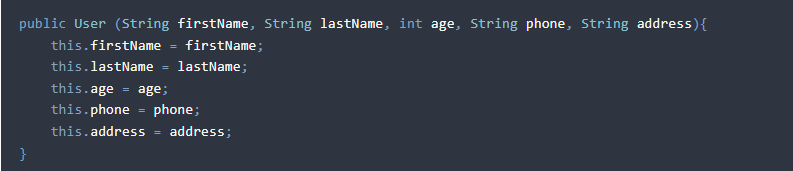
\includegraphics[width=\textwidth]{fig/Builder/UserNormalDesign.png}
\end{figure}\\[0.1in]
Vậy chuyện gì xảy ra nếu ta không bắt buộc 3 trường tuổi, số điện thoại và địa chỉ? Khi đó sẽ xảy ra vấn đề. Ta cần nhiều hàm dựng hơn và dẫn đến tình trạng \textbf{telescoping constructors}. Nói cách khác, cách thiết kế này sẽ mất tính thẩm mĩ và rất là rối
\begin{figure}[!htb]
    \centering
    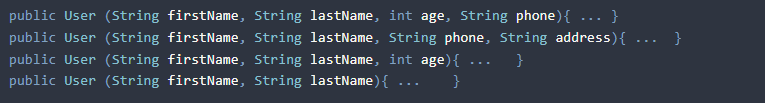
\includegraphics[width=\textwidth]{fig/Builder/UglyDesign.png}
\end{figure}\\[0.1in]
\textbf{Builder Pattern} sinh ra để khắc phục vấn đề này. Nó giúp ta có thể tạo lớp immutable kiểm soát một đối tượng phức tạp có số lượng thuộc tính đủ lớn
\section{Định nghĩa và Mô hình cấu trúc}
\subsection{Định nghĩa}
\textbf{Builder Pattern} là một pattern tách biệt cách dựng của một đối tượng phức tạp khỏi sản phầm cuối cùng. Bằng cách này, cùng một cách dựng có thể tạo ra nhiều sản phẩm khác nhau. Cũng như \textbf{Factory Pattern}, \textbf{Builder Pattern} thuộc nhóm \textbf{Creational Pattern} (Nhóm khởi tạo)
\section{Mô hình cấu trúc}
Mô hình cấu trúc của Builder Pattern được mô tả như sau:
\begin{figure}[!htb]
    \centering
    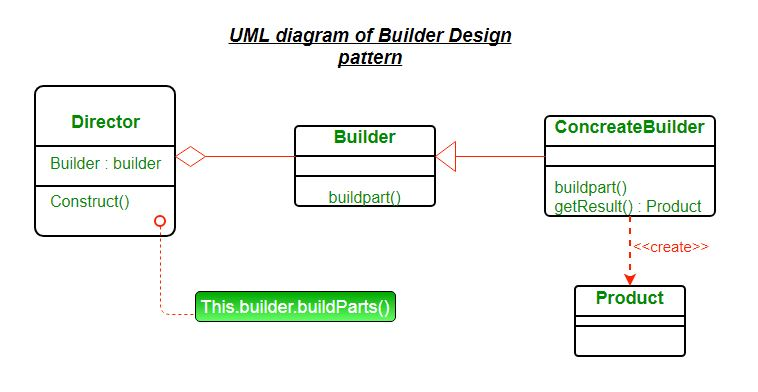
\includegraphics[width=\textwidth]{fig/Builder/BuilderDiagram.png}
    \caption{Mô hình cấu trúc Builder Pattern}
\end{figure}
Trong đó:
\begin{itemize}
    \item \textbf{Product}: Là lớp định nghĩa đối tượng phức tạp để được sinh ra từ builder pattern
    \item \textbf{Builder}: Là lớp trừu tượng định nghĩa các bước cần thiết để tạo sản phẩm đúng cách
    \item \textbf{Concreate Builder}: Là những lớp được kế thừa từ \textbf{Builder}. Những lớp này chứa chức năng để tạo một đối tượng phức tạp cụ thể
    \item \textbf{Director}: Là lớp đảm nhận thuật toán sinh ra sản phẩm cuối cùng
\end{itemize}

\section{Cài đặt}
Áp dụng \textbf{Builder Pattern} để giải quyết vấn đề ở mục 1. Về ý tưởng, ta lồng thêm lớp \textbf{UserBuilder} vào trong lớp \textbf{User} để hỗ trợ việc tạo đối tượng mà không mất đi tính immutability
Dưới đây là code minh họa:
\newpage

\begin{figure}[!htb]
    Lớp \textbf{User}:
    \centering
    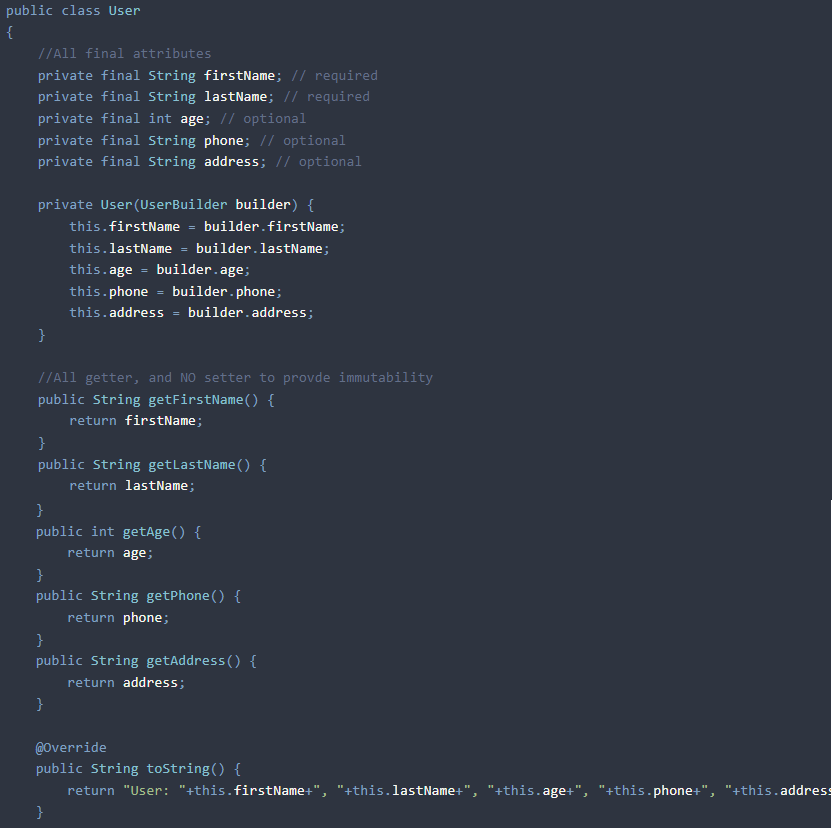
\includegraphics[width=\textwidth]{fig/Builder/UserPart1.png}
\end{figure}

\begin{figure}
    Lớp \textbf{UserBuilder} trong lớp \textbf{User}
    \centering
     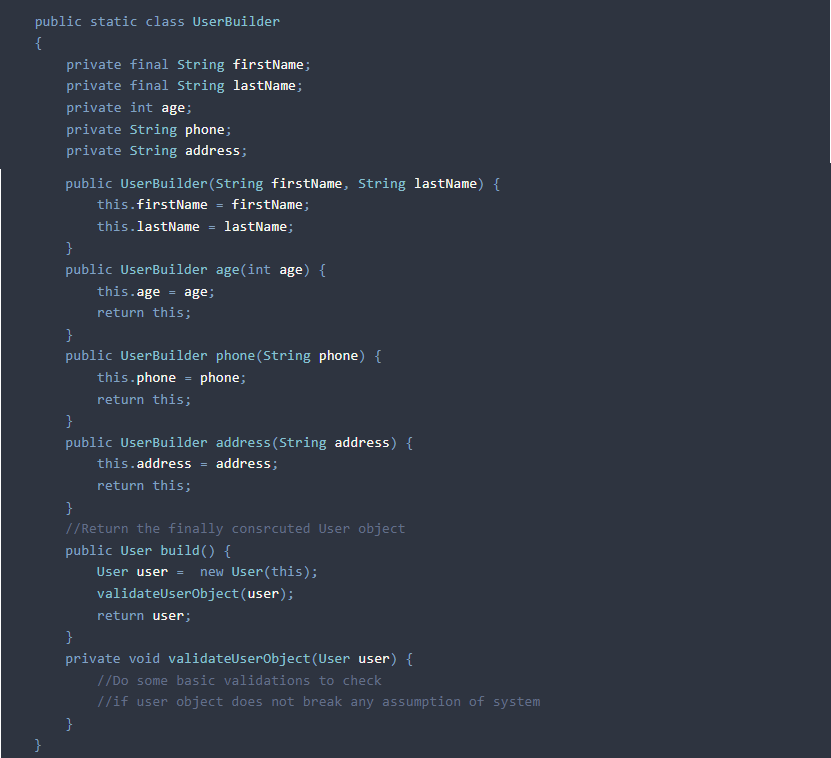
\includegraphics[width=\textwidth]{fig/Builder/UserPart2.png}
\end{figure}

\begin{figure}[!htb]
    Lớp Client để xây dựng các đối tượng bằng \textbf{UserBuilder}:
    \centering
    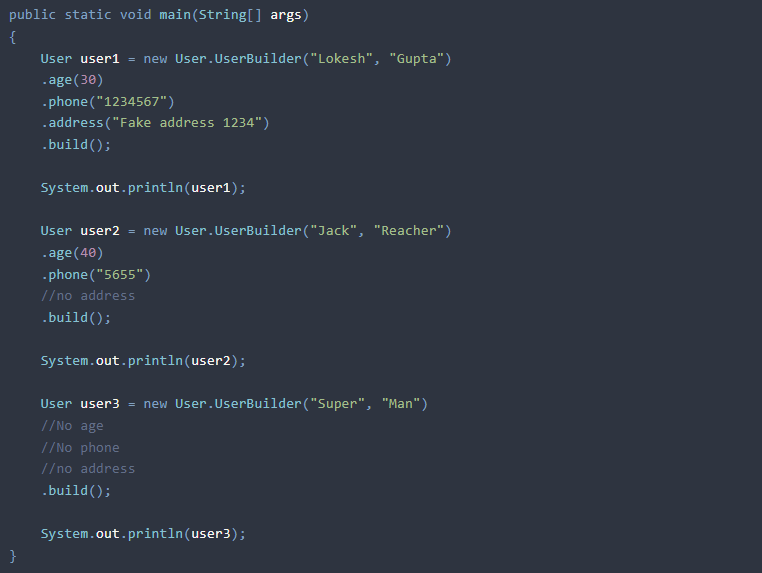
\includegraphics[width=\textwidth]{fig/Builder/main.png}
\end{figure}

\newpage

\section{Thực tế}
\textbf{RTF Converter} (Rich Text Format Converter - bộ chuyển đổi văn bản sang nhiều định dạng khác nhau) có khối xây dựng text sử dụng builder để lưu trữ text trong định dạng RTF\\[0.1in]
\textbf{Builder} là một pattern phổ biến trong Smalltalk-80[Par90]:
\begin{itemize}
    \item Lớp Parser trong hệ thống con biên dịch là \textbf{Director}. Nó lấy đối tượng ProgramNodeBuilder làm đối số. Một đối tượng Parser thông báo đối tượng  ProgramNodeBuilder mỗi lần nó nhận diện một cấu trúc cú pháp. Khi nào trình phân tích cú pháp được thực hiện, nó yêu cầu builder cho cây phân tích cú pháp mà nó đã xây dựng và trả về cho Client
    \item ClassBuilder là một builder mà các lớp sử dụng để tạo các lớp con cho chính chúng. Trong trường hợp này một lớp vừa là \textbf{Director} vừa là \textbf{Product}
    \item ByteCodeStream là một builder tạo ra một phương thức đã được biên dịch như một mảng byte. ByteCodeStream là một cách dùng khác của \textbf{Builder Pattern} vì đối tượng phức tạp nó tạo được mã hóa thành một mảng byte, không như một đối tượng Smalltalk thông thường. Nhưng interface của ByteCodeStream là một trường hợp điển hình của builder và sẽ dễ dàng thay thế ByteCodeStream bằng một lớp khác đại diện chương trình như một đối tượng composite
\end{itemize}